\sisetup{per-mode=symbol}
% Aufrechtes mathematisches Mikrozeichen, passend zur Einheitenschrift.
\DeclareSIPrefix{\micro}{\ensuremath{\upmu}}{-6}
\chapter{Sensoren}\label{ch:chapter_03}
\section{Distanzmessung mit Ultraschall}\label{sec:Ultraschall}
Sensoren sind technische Bauteile, die es ermöglichen, die physikalische Umgebung eines Roboters zu erfassen. Die Messwerte werden in elektrische Signale umgewandelt, die vom Mikroprozessor des Roboters verarbeitet werden können. In diesem Kapitel werden Sie die Funktionsweise von Ultraschallsensoren kennenlernen.

Der Ultraschallsensor HC-SR04 besitzt einen Sender (Trigger) und einen Empfänger (Echo), die ähnlich wie bei einer Fledermaus funktionieren (Mund = Trigger; Ohren = Echo).

\begin{center}
    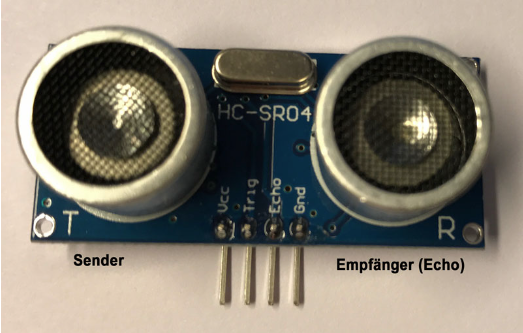
\includegraphics[width = 0.3\textwidth]{FF/Robotik/Skript/Abbildungen/ultraschallsensorHC-SR04.png}
\end{center}

Der Ultraschallsensor sendet ein Schallsignal mit ca. \qty{40}{\kilo\hertz}. Damit ist er zu hochfrequent, um von Menschen gehört zu werden --- Katzen und Hunde könnten ihn jedoch hören.

Die Messung wird ausgelöst, indem man den Trigger-Pin für mindestens \qty{10}{\micro\second} auf HIGH setzt und dann auf LOW. Kurze Zeit nach dem Abfall des Triggers werden 8 Schallimpulse gesendet. Sofort danach geht der Echo-Pin auf einen HIGH-Pegel und wartet auf den Empfang des akustischen Echos. Sobald das Echo empfangen wurde, fällt der Ausgang am Echo auf den LOW-Pegel.

\begin{center}
    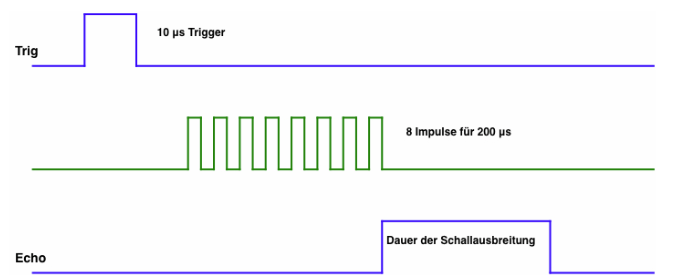
\includegraphics[width = 0.5 \textwidth]{FF/Robotik/Skript/Abbildungen/PinZustandMessung.png}
\end{center}

Um die Pulslänge am Echo-Eingang zu messen, wird die Funktion \lstinline|pulseIn(ECHO_PIN, HIGH)| verwendet. Diese gibt an, wie lange (in \unit{\micro\second}) das Signal am ECHO\_PIN auf HIGH war.


Die Distanz \(d\) berechnet sich dann aus der Zeit \(t\) vom Aussenden des Signals bis zu seiner Rückkehr, wobei zu beachten ist, dass das Schallsignal in dieser Zeit den Weg zwischen Sensor und Hindernis zweimal zurücklegt.
\begin{center}
    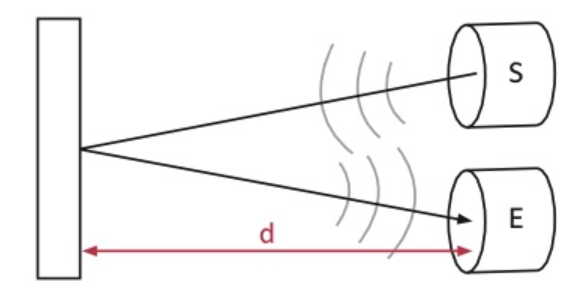
\includegraphics[width = 0.25\textwidth]{FF/Robotik/Skript/Abbildungen/laufzeitmessung.png}
\end{center}

Es gilt also :
\[
    d = \frac{c \cdot t}{2}.
\]
Wenn man nun berücksichtigt, dass Arduino die Zeit \(t\) in \unit{\micro\second} misst und mit der Schallgeschwindigkeit \(c\approx \qty{343}{\metre\per\second} = \qty{0.0343}{\centi\metre\per\micro\second}\) erhält man:

\[
    d = \frac{c \cdot t}{2} \approx \frac{\qty{0.0343}{\centi\metre\per\micro\second}}{2}\cdot t \unit{\micro\second} \approx \frac{t}{58} \unit{\centi\metre}
\]



\begin{myexercise}
    \begin{aenum}
        \item Stecken Sie den Ultraschallsensor auf das Breadbord und verbinden Sie es mit dem Arduino. Verwenden Sie die digitalen Pins 7 und 6 für \lstinline|Trig| und \lstinline|Echo|.
              \begin{center}
                  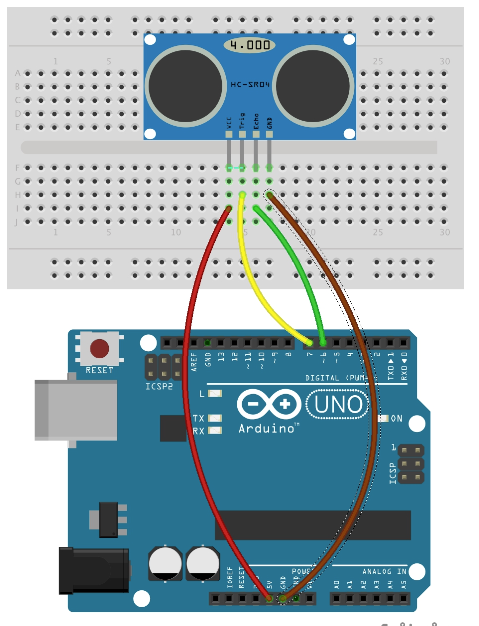
\includegraphics[width = 0.25\textwidth]{FF/Robotik/Skript/Abbildungen/SchaltkreisUltraschall.png}
              \end{center}

        \item  Laden Sie das Programm \hyperref[lst:ultraschall-intro]{\texttt{Intro\_Ultraschall.ino}} von Moodle herunter und testen Sie den Sensor.
              % \item Die Distanz in Zentimeter wird berechnet, indem man die Zeit in Mikrosekuneden durch 58 teilt. Weisen Sie nach, dass diese Distanzberechnung mit der \Cref{eq:distanzberechnung} übereinstimmt.
        \item \textbf{Verbesserungen:} Der Ultraschallsensor ist nur im Bereich 2 cm bis 3 m zuverlässig. Verbessern Sie Ihr Programm so, dass die Distanzmessung nur ausgegeben wird, wenn der gemessene Wert in diesem Bereich liegt, andernfalls soll \enquote{nicht im Messbereich} ausgegeben werden. Verwenden sie dazu die \lstinline|if|-Anweisung der Form:

              \begin{lstlisting}
    if (Bedingung1 && Bedingung2)
    {
        Anweisungen, die ausgeführt werden, wenn beide Bedingungen erfüllt sind
    }
    else
    {
        Anweisungen, die ausgeführt werden, wenn mindestens eine der Bedingungen nicht erfüllt ist 
    }
\end{lstlisting}
    \end{aenum}

    \begin{myremark}
        In Arduino (C++) werden logische Verknüpfungen mit speziellen Operatoren geschrieben:
        \[
            \begin{array}{c|c|c}
                \text{Bedeutung} & \text{Operator} & \text{Beispiel}           \\ \hline
                \text{UND}       & \texttt{\&\&}   & \texttt{a > 0 \&\& b > 0} \\
                \text{ODER}      & \texttt{||}     & \texttt{a > 0 || b > 0}   \\
                \text{NICHT}     & \texttt{!}      & \texttt{!(a > 0)}
            \end{array}
        \]
        Der Operator \texttt{!} kehrt den Wahrheitswert einer Bedingung um.

    \end{myremark}



\end{myexercise}




% \begin{myexercise}\label{ex:UltraschallBetrieb}
%     Schreiben Sie ein Programm zur Entfernungsmessung.
%     \begin{enumerate}
%         \item \textbf{Variablen festlegen:} Wir benötigen vier Variablen:
%               \begin{lstlisting}
%                         const int TRIG_PIN = 7;
%                         const int ECHO_PIN = 6;
%                         unsigned long duration;
%                         float distance_cm;
%                     \end{lstlisting}
%             %   Die beiden Variablen \lstinline|TRIG_PIN| und \lstinline|ECHO_PIN| bezeichnen die Arduino-Pins, an welchen der Sensor angeschlossen ist. Passen Sie diese an Ihren Aufbau an. \newline
%               In die Variable \lstinline|duration| soll die gemessene Zeit gespeichert werden. \newline
%               Die aus der Zeit berechnete Distanz soll in die Variable \lstinline|distance_cm| gespeichert werden.
%         \item \textbf{Setup:} Trigger muss auf OUTPUT und ECHO auf INPUT initialisiert werden. Ausserdem soll die USB-Verbindung zum Computer verwendet werden \lstinline|Serial.begin(9600).|
%         \item \textbf{Loop:}
%               \begin{enumerate}
%                   \item   In der Schleife soll der Trigger-Pin für 10 Mikrosekunden auf HIGH gesetzt werden und anschliessend wieder auf LOW, um die Messung auszulösen. Da die \lstinline|delay|-Funktion in Millisekunden rechnet, benötigen Sie eine andere Warte-Funktion:
%                         \begin{lstlisting}
%             delayMicroseconds(10)
%         \end{lstlisting}
%                   \item Verwenden Sie dann den Befehl \lstinline|duration = pulseIn(ECHO_PIN, HIGH)|, um die verstrichenen Mikrosekunden in die Variable \lstinline|duration| zu speichern.
%                   \item Lassen Sie die gemessenen Werte auf dem Computer anzeigen mit
%                         \begin{lstlisting}
%             Serial.print("duration = ");
%             Serial.print(duration);
%             Serial.println(" Mikrosekunden");
%         \end{lstlisting}
%                   \item Fügen Sie am Schluss des Loops eine Wartezeit von 500 ms ein, damit nur jede halbe Sekunde eine Messung durchgeführt wird. Testen Sie anschliessend Ihr Programm.
%               \end{enumerate}

%         \item \textbf{Distanzberechnung:}
%               \begin{enumerate}
%                   \item Verwenden Sie die Formel und die Schallgeschwindigkeit in der Theorie oben, um die Distanz zu berechnen.
%                   \item Lassen Sie auch die Werte der Distanz auf dem Computer ausgeben und testen Sie Ihr Programm.
%               \end{enumerate}
%         \item \textbf{Verbesserungen:} Der Ultraschallsensor ist nur im Bereich 2 cm bis 3 m zuverlässig. Verbessern Sie Ihr Programm so, dass die Distanzmessung nur ausgegeben wird, wenn der gemessene Wert in diesem Bereich liegt.
%     \end{enumerate}
%     \begin{myanswer}
%         \lstinputlisting{FF/Robotik/Skript/Code/Intro_Ultraschall-lsg/Intro_Ultraschall-lsg.ino}
%     \end{myanswer}
% \end{myexercise}


Für die folgenden Aufträge benötigen Sie den Roboter. Dieser hat einen anderen Ultraschallsensor eingebaut, weshalb die folgenden Programme mit dem HC-SR04 nicht funktionieren.

\begin{center}
    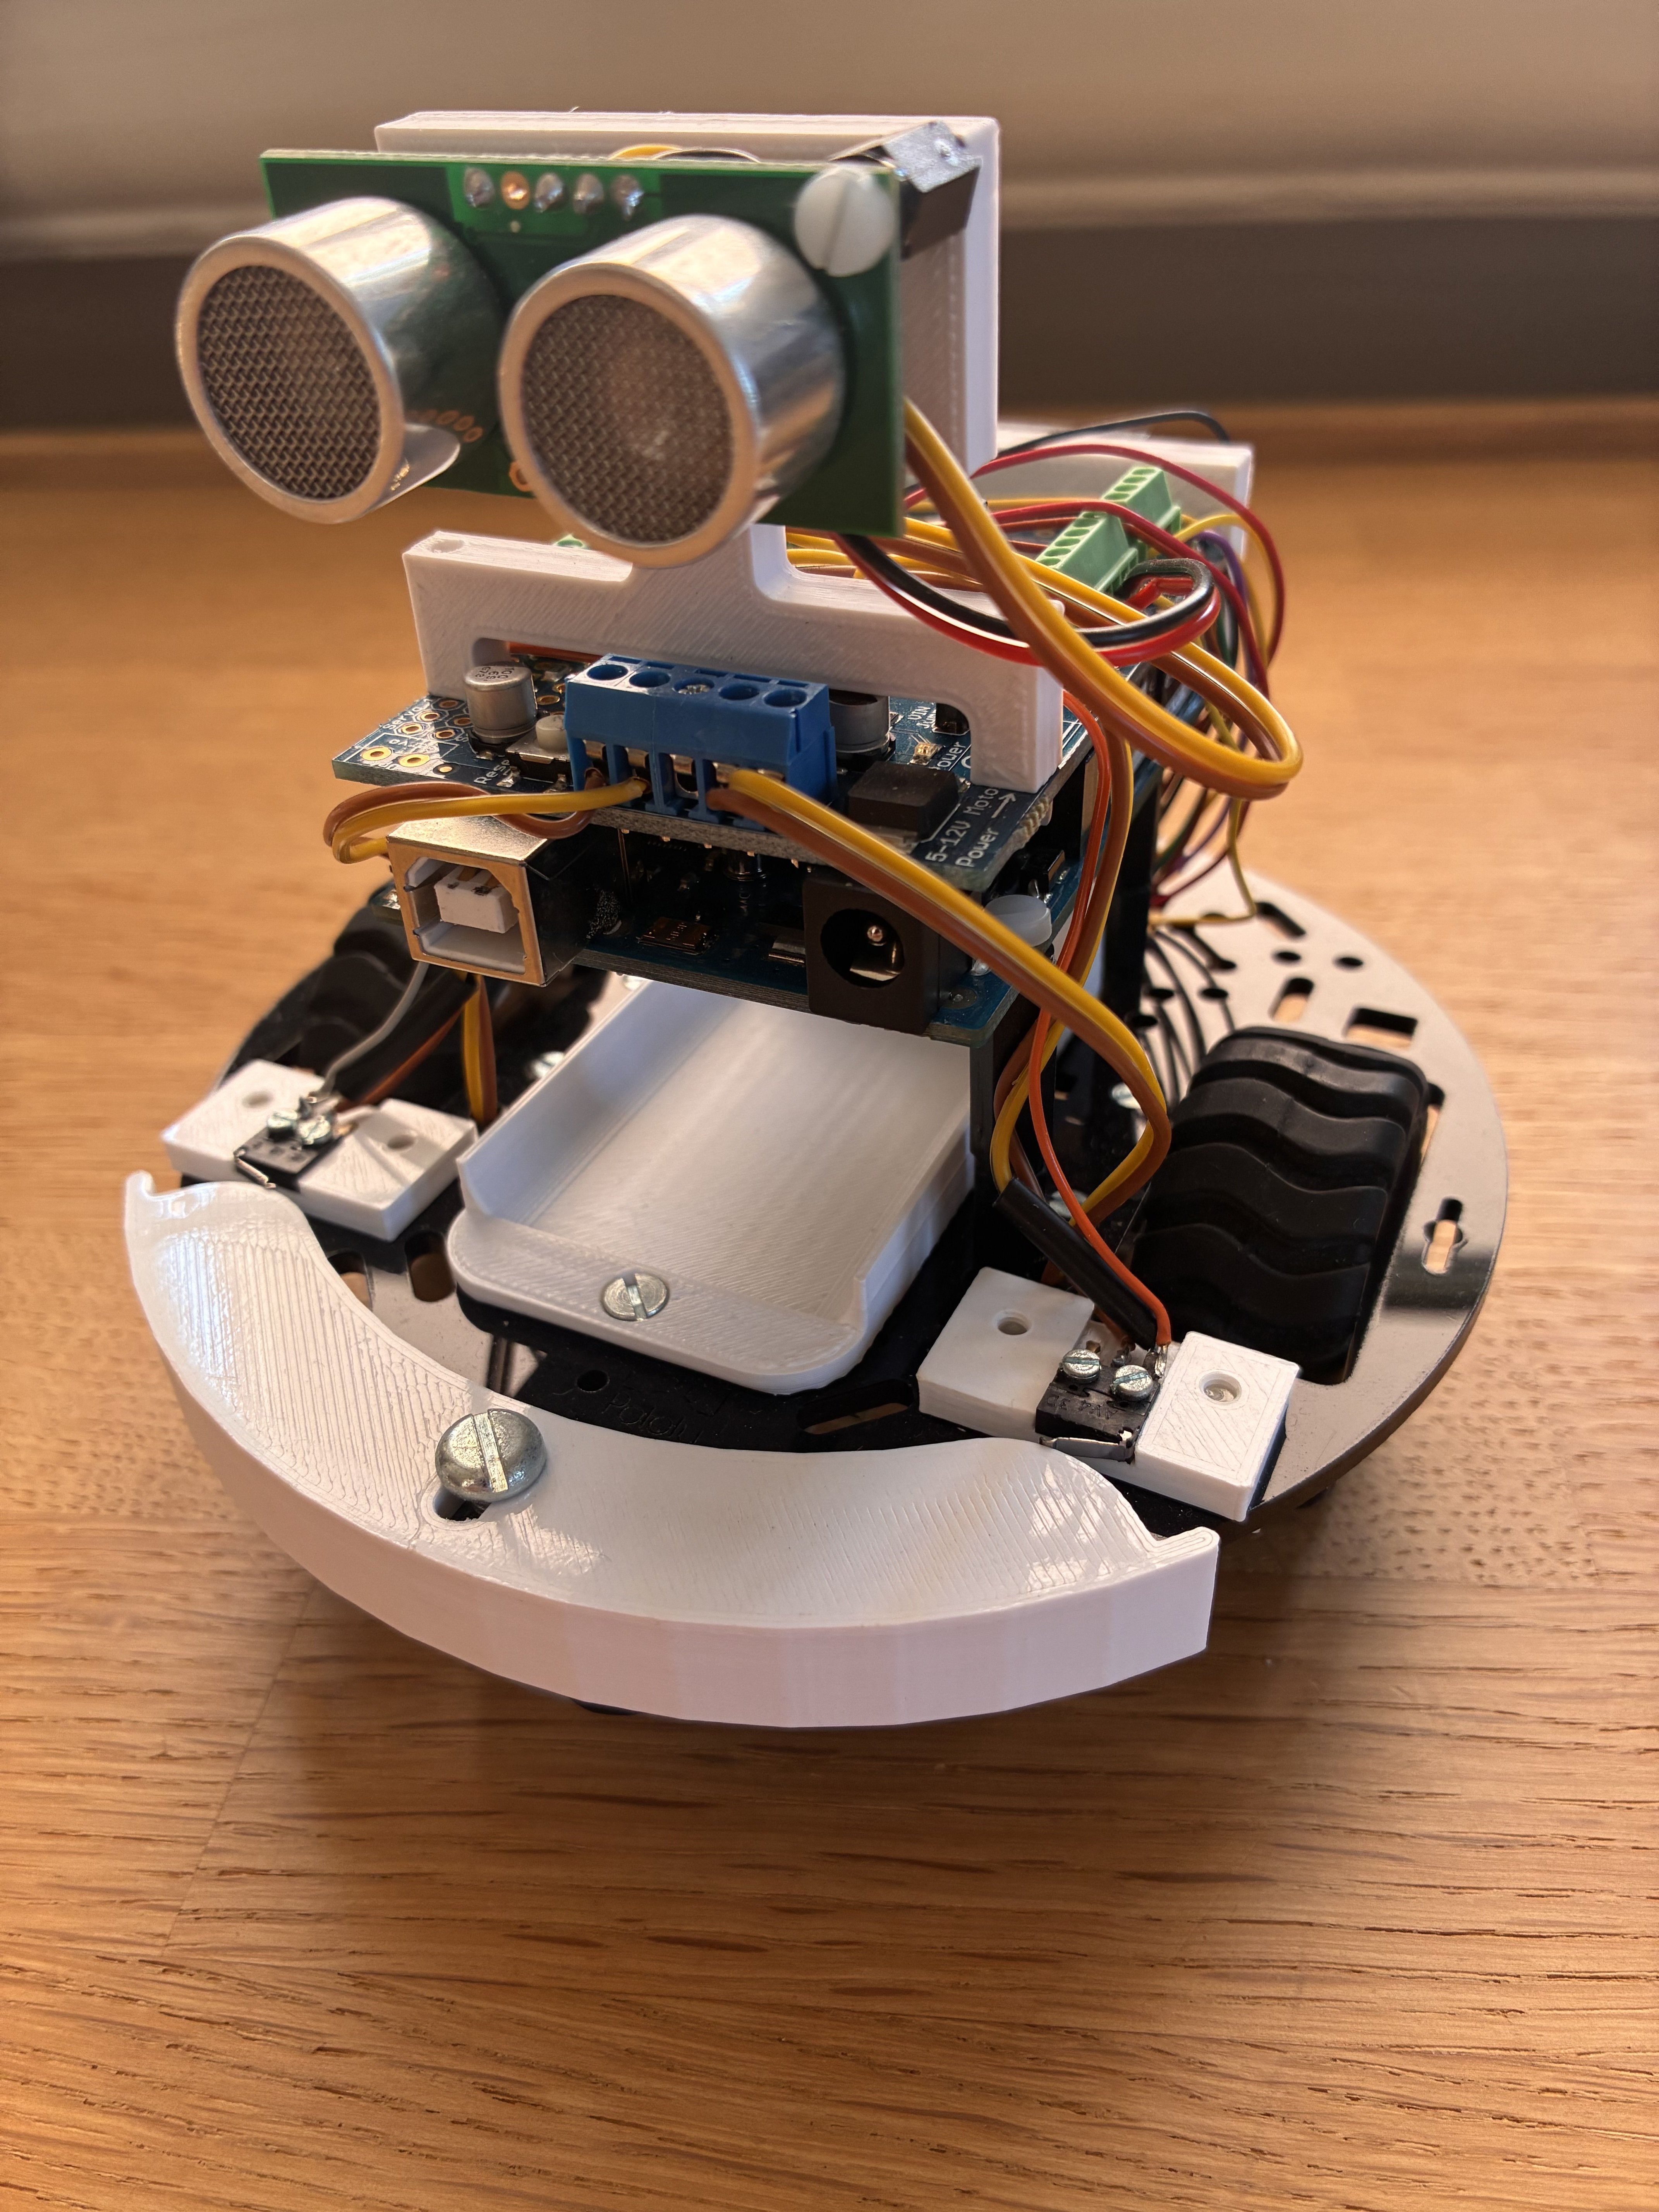
\includegraphics[width = 0.25\textwidth]{FF/Robotik/Skript/Abbildungen/roboter.jpg}
\end{center}
Durch die Verwendung von \enquote{Libraries} kann die Bedienung von Sensoren und die Lesbarkeit von Programmcode vereinfacht werden. Für den Ultraschallsensor gibt es eine Library, mit welcher man den Abstand mit einem einzigen Befehl messen kann. Im Hintergrund werden jedoch genau die gleichen Schritte durchgeführt, wie in der vorherigen Aufgabe.

Die entsprechende Library sollten Sie bereits letzte Woche installiert haben. Falls nicht, können Sie das Zip-File \texttt{LibrariesFuerFreifach2026} von Moodle herunterladen und in Ihrem Ordner Arduino/libraries entpacken.
\begin{myexercise}

    %     \begin{enumerate}
    %         \item Laden Sie von Moodle das Zip-File \texttt{LibrariesFuerFreifach2026} herunter.
    %         \item Entpacken Sie das Zip-File in Ihrem Ordner Arduino/libraries
    %      \end{enumerate}
    Laden Sie das Programm \hyperref[lst:ultraschall-roboter]{\texttt{ultraSonicTest1}} von Moodle herunter.
    \newline
    Beachten Sie, wie die einzelnen Schritte aus dem vorherigen Programm nun in der Funktion \lstinline|readSensorValue()| zusammengefasst sind.
    \begin{aenum}
        \item Testen Sie das Programm mit dem Roboter (nicht mit dem HC-SR04).
        \item \emph{Freiwillig:} Am Anfang des Programms wird mit \lstinline|#include <USSensor.h>| die Bibliothek \lstinline|USSensor| geladen. Darin sind alle Befehle aufgeführt, die von der Library zur Verfügung gestellt werden. Deren implementierung findet man in der Datei \texttt{USSensor.cpp}. Öffnen Sie diese Datei auf Ihrem Computer (in der Regel ist sie im Ordner \lstinline|/Documents/Arduino/libraries/|). Suchen Sie darin nach dem Code, der die Messung auslöst (Trigger für \qty{10}{\micro\second} auf HIGH) und den Abstand berechnet (Zeit / 58).
    \end{aenum}

\end{myexercise}

Kombinieren Sie den Ultraschallsensor mit den Motoren des Roboters.

\begin{myexercise}
    Programmieren Sie den Roboter so, dass er sich jedes Mal um grob \(180^\circ\) dreht, wenn er ein Hindernis erkannt hat, das sich weniger als 10 cm vor ihm befindet. So sollte sich der Roboter im Zimmer bewegen können, ohne dass er in eine Wand fährt.

    Verwenden Sie dazu die Datei \hyperref[lst:hinundher-template]{\texttt{hinundher\_template.ino}} von Moodle. Diese enthält bereits die Funktionen \lstinline|vorwaerts()|, \lstinline|stoppen()| und \lstinline|drehen()|, die Sie verwenden können. Den Drehwinkel können Sie über die Konstante \lstinline|ROTATION_TIME| steuern, die angibt, wie lange in \unit{\milli\second} sich der Roboter um die eigene Achse dreht.

    Bemerkung: \newline
    Damit das Programm nicht unendlich lange läuft, ist die Anweisung im Setup-Block eingefügt. Im Gegensatz zum Loop-Block wird dieser Befehl nur einmal ausgeführt, wenn der Arduino gestartet wird. Die Anweisung ist aber so konzipiert, dass der Roboter erst nach 5 Drehungen stoppt. Sie können die Anzahl Drehungen in der Variable \lstinline|MAX_ANZAHL_DREHUNGEN| anpassen.

\end{myexercise}

\begin{myexercise}
    Führen Sie den Roboter spazieren!\newline
    Schreiben Sie ein Programm, das bewirkt, dass der Roboter Ihrer Hand folgt. Wenn der Roboter eine Distanz misst, die grösser oder gleich 20 \unit{\centi\metre} ist, soll der er vorwärts fahren. Wenn die gemessene Distanz kleiner ist, soll er rückwärtsfahren.

    Tipp: Ergänzen Sie die Funktionen aus \hyperref[lst:hinundher-template]{\texttt{hinundher\_template.ino}} mit einer Funktion \lstinline|void rueckwaertsFahren(int speed)|
\end{myexercise}
\begin{myexercise}
    Optimieren Sie den Roboter Spaziergang! \newline
    Wenn der gemessene Abstand grösser als 50 \unit{\centi\metre} oder kleiner als 10  \unit{\centi\metre} ist, soll der Roboter stehen bleiben.

    Tipp: Sie kennen vermutlich die Python Verzweigung der Form \lstinline[language=Python]|if ... elif ... else|. In C++ lautet die Syntax wie folgt:
    \begin{lstlisting}
    if (Bedingung 1) {
            Anweisungen;
        }
    else if (Bedingung 2) {
            Anweisungen;
        }
    else {
            Anweisungen;
        }
     \end{lstlisting}

\end{myexercise}
\begin{myexercise}
    Schreiben Sie ein Programm, mit dem der Roboter parallel zu einer Wand in einem Abstand von  20 \unit{\centi\metre} fährt. Überlegen Sie sich eine Strategie, wie der Roboter diesen Abstand einhalten kann.
\end{myexercise}

% Wie genau misst der Ultraschallsensor?

% Für die folgende Aufgabe benötigen Sie zusätzlich
% \begin{itemize}
%     \item ein Buch oder ein ähnliches Hindernis
%     \item ein Massband
%     \item ein Geodreieck
%     \item und eine Schachtel.
% \end{itemize}
\begin{myexercise}
    Untersuchen Sie die Messgenauigkeit des Ultraschallsensors.
    \begin{aenum}
        % \item  Stellen Sie ein Hindernis auf und vergleichen Sie den tatsächlichen Abstand (Massband) mit dem Messwert des Ultraschalls. In welchem Bereich misst der Sensor die Distanz korrekt?
        \item Stellen Sie ein Hindernis in einem bestimmten Abstand vor den Roboter (z.B. 30 cm). Drehen Sie das Hindernis schrittweise um \(10^\circ\), sodass das Schallsignal auf eine schräge Wand trifft. In welchem Winkelbereich wird der Abstand korrekt gemessen?
        \item Stellen Sie den Roboter in eine Schachtel. Schreiben Sie ein Programm, das den Roboter wiederholt um etwa \(10^\circ\) dreht und nach jeder Drehung eine Distanzmessung durchführt.
        \item Wie \enquote{sieht} der Roboter die Schachtel? Fügen Sie die gemessenen Distanzen aus der Aufgabe davor in das Python-Programm \hyperref[lst:polarkoord-sketch]{\texttt{polarkoord-sketch}} ein, das Sie auf Moodle finden.
    \end{aenum}
    % \lstinputlisting{FF/Robotik/Skript/Code/polarkoord_sketch.py}
    % \begin{myanswer}
    %     \lstinputlisting{FF/Robotik/Skript/Code/schachtel/schachtel.ino}
    % \end{myanswer}
\end{myexercise}


\clearpage

\section{Weitere Sensoren des Roboters}
\subsection{Distanzmessung mit Infrarot}
Auf der Rückseite besitzt der Roboter einen Infrarot-Sensor zur Distanzmessung. Dieser funktioniert ein wenig anders als der Ultraschall-Sensor.

Bei der Infrarot-Distanzmessung wird ein unsichtbarer Lichtstrahl ausgesendet. Dieser wird an einem Objekt reflektiert und über eine Linse auf einen Detektor gelenkt. Je nach Entfernung des Objekts trifft das reflektierte Licht an einer anderen Stelle auf den Detektor. Letzterer ist so konstruiert, dass je nach Position des einfallenden Lichts eine andere Spannung erzeugt wird. Aus der gemessenen Spannung kann schliesslich die Distanz ermittelt werden.

\begin{center}
    % 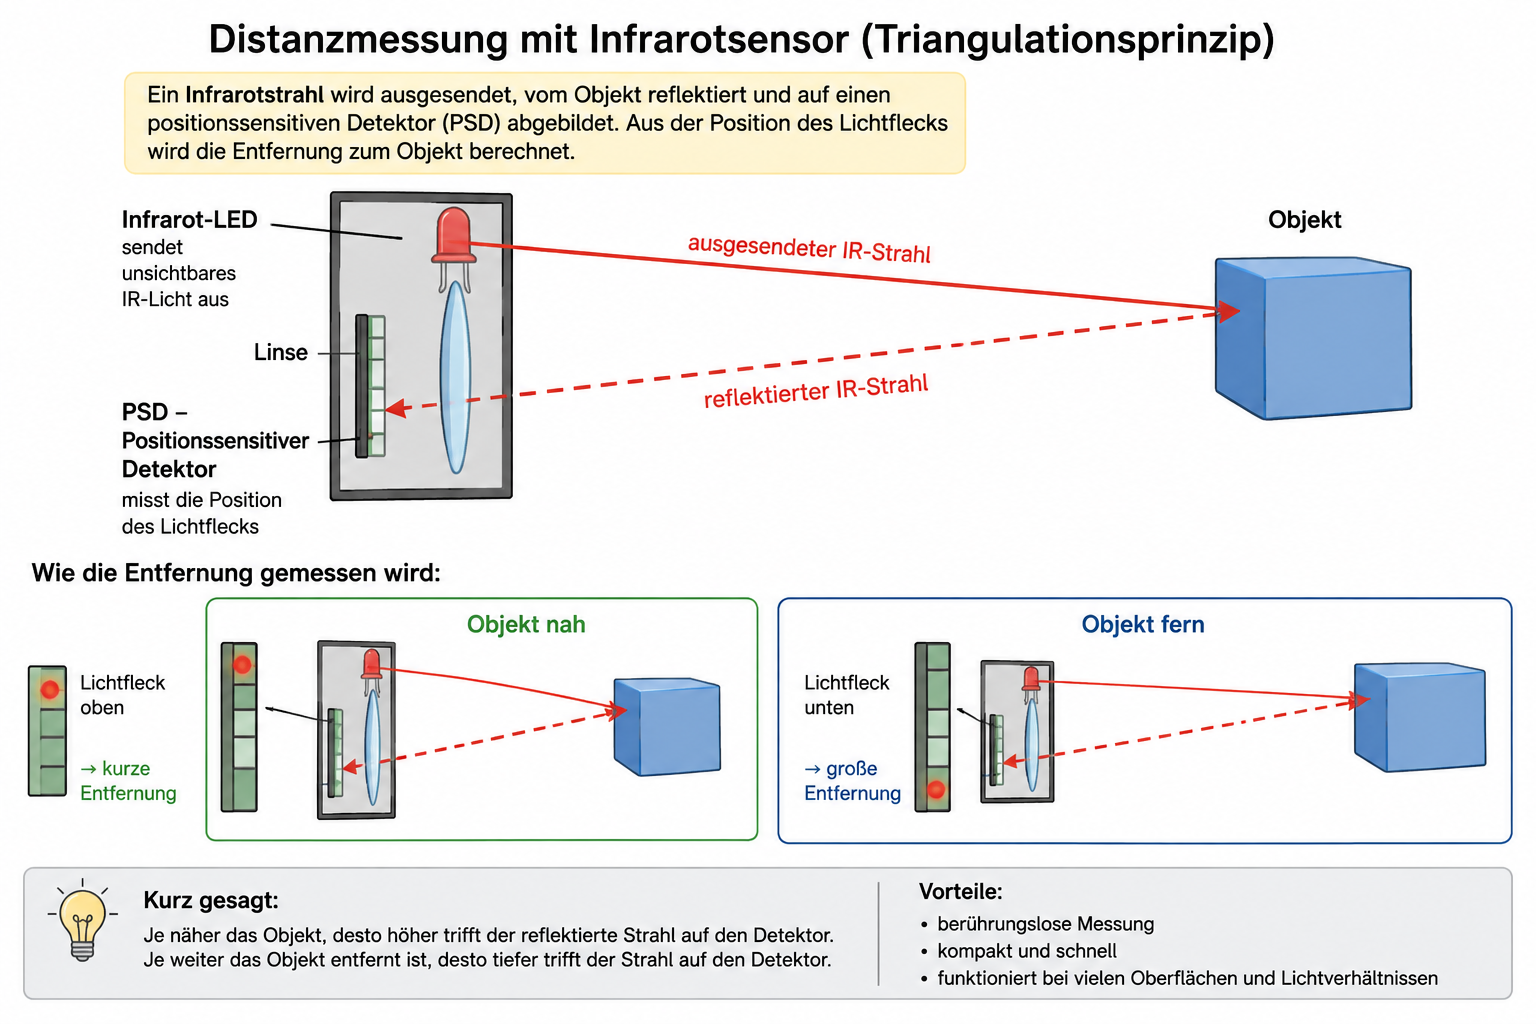
\includegraphics[width = 0.75\textwidth]{FF/Robotik/Skript/Abbildungen/Infrared-distance.png}
    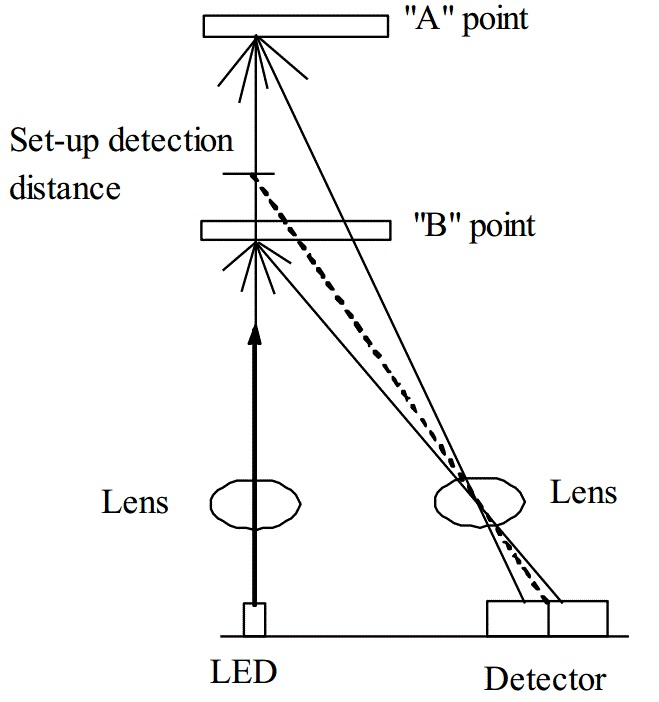
\includegraphics[width = 0.55\textwidth]{FF/Robotik/Skript/Abbildungen/Sharp_depth_sensor.jpg}
\end{center}

Für die Aufträge benötigen Sie das folgende Material:
\begin{itemize}
    \item Roboter
    \item Massband
    \item Hindernis (Buch)
    \item Schachtel
\end{itemize}

\begin{myexercise}
    Der Sensor muss zuerst kalibriert werden. Verwenden Sie dazu das Programm \hyperref[lst:infrarot-test]{\texttt{infraRedTest}}, das Sie auf Moodle finden. Stellen Sie den Roboter in verschiedenen Abständen zu einem Hindernis auf und notieren Sie die gemessenen Werte in die folgende Tabelle.
    \begin{center}
        \begin{tabular}{c|c}
            \(d\) in cm & irValue \\
            \hline
            5           &         \\
            10          &         \\
            15          &         \\
            20          &         \\
            25          &         \\
            30          &         \\
        \end{tabular}
    \end{center}
\end{myexercise}

\begin{myexercise}
    Es gibt nicht DIE Formel, mit der man den gemessenen Wert in einen Abstand umwandeln kann. Einigermassen gute Resultate soll man aber mit dieser Berechnung erhalten:
    \begin{lstlisting}
        float distance_cm = (2914.0 / (irValue + 5) ) - 1;
    \end{lstlisting}
    Testen Sie, wie gut diese Formel zu Ihren Messwerten passt.
\end{myexercise}

\begin{myexercise}
    Der ängstliche Roboter!\newline
    Schreiben Sie ein Programm, mit dem der Roboter flieht, wenn sich ihm etwas von hinten nähert. \newline
    Zusatz: Je kleiner der Abstand zum Objekt ist, desto schneller soll der Roboter fliehen.
\end{myexercise}

\begin{myexercise}
    Testen Sie, wie gut sich der IR-Sensor im \enquote{Schachtel-Experiment} macht:
    \begin{aenum}
        \item Stellen Sie den Roboter in eine Schachtel. Schreiben Sie ein Programm, das den Roboter wiederholt um etwa \(10^\circ\) dreht und nach jeder Drehung eine Distanzmessung durchführt.
        \item Wie \enquote{sieht} der Roboter die Schachtel? Fügen Sie die gemessenen Distanzen in das  Python-Programm \hyperref[lst:polarkoord-sketch]{\texttt{polarkoord-sketch}} ein, das Sie auf Moodle finden.
    \end{aenum}

\end{myexercise}

\begin{myremark}
    Der Infrarotsensor hat zwar gegenüber dem Ultraschallsensor den Nachteil, dass er kalibriert werden muss, da der gemessene Sensorwert nicht direkt einer bestimmten Distanz entspricht. Dafür kann der Infrarotsensor den Abstand deutlich schneller und häufiger messen. Dies ist besonders nützlich, wenn der Roboter schnell auf Veränderungen in seiner Umgebung reagieren soll.
\end{myremark}

\clearpage

\subsection{Berührungssensoren}
In diesem Kapitel werden Sie die letzten beiden Sensoren des Roboters kennenlernen.

\begin{myexercise}
    \begin{aenum}
        \item Testen Sie den Touchsensor des Roboters mit dem Programm \hyperref[lst:touchsensor-test]{\texttt{TouchSensorTest.ino}} (von Moodle downloaden).
        \item Programmieren Sie den Roboter so, dass er vorwärts fährt. Wenn der Touchsensor eine Kollision meldet, soll sich der Roboter einige cm zurückbewegen, sich vom Hindernis wegdrehen (Drehrichtung je nach Kollisionsstelle) und dann weiterfahren.
    \end{aenum}
\end{myexercise}
\subsection{Lichtsensoren}
An der Unterseite des Roboters befindet sich zwei Lichtsensoren. Diese können messen, ob sich unter ihnen ein heller oder dunkler Untergrund befindet.

\begin{myexercise}
    \begin{aenum}
        \item Testen Sie die Lichtsensoren des Roboters mit dem Programm \hyperref[lst:lichtsensor-test]{\texttt{LightSensorTest.ino}} (von Moodle downloaden).
        \item Programmieren Sie den Roboter so, dass er einer schwarzen Linie auf hellem Untergrund folgt.\newline
              Tipps:
              \begin{itemize}
                  \item Schreiben Sie zwei Funktionen \lstinline|linkskurve()|
                        und \lstinline|rechtskurve()|, mit denen der Roboter
                        eine Links- bzw. Rechtskurve fährt.

                  \item Wenn der linke Sensor einen hellen Untergrund erkennt,
                        soll der Roboter eine Rechtskurve fahren. Wenn der rechte
                        Sensor einen hellen Untergrund erkennt, soll er eine
                        Linkskurve fahren.
                  \item Überlegen Sie auch, was der Roboter tun soll, wenn beide Sensoren
                        einen dunklen bzw. beide einen hellen Untergrund erkennen.
              \end{itemize}

    \end{aenum}
\end{myexercise}


\clearpage

\section{Braitenberg-Vehikel}
Braitenberg-Vehikel sind einfache Roboter, die mit Sensoren ihre Umgebung wahrnehmen und darauf reagieren. Die Sensoren sind dabei direkt oder über einfache Regeln mit den Motoren verbunden. Je nach Verschaltung können die Roboter beispielsweise auf eine Lichtquelle zufahren, vor ihr fliehen oder Hindernissen ausweichen. Obwohl die Steuerung sehr einfach aufgebaut ist, kann das Verhalten der Roboter überraschend komplex und zielgerichtet wirken. Braitenberg-Vehikel zeigen damit anschaulich, wie aus einfachen Regeln komplexes Verhalten entstehen kann.

\subsection{Vehikel Furcht und Aggression}
Diese Vehikel besitzen je zwei Motoren und zwei Sensoren. Je stärker der Sensorwert, desto schneller drehen die Motoren. Die beiden Arten \enquote{Furcht} und \enquote{Aggression} unterscheiden sich jedoch in der Art, welcher Sensorwert welchen Motor beeinflusst:

\begin{center}
    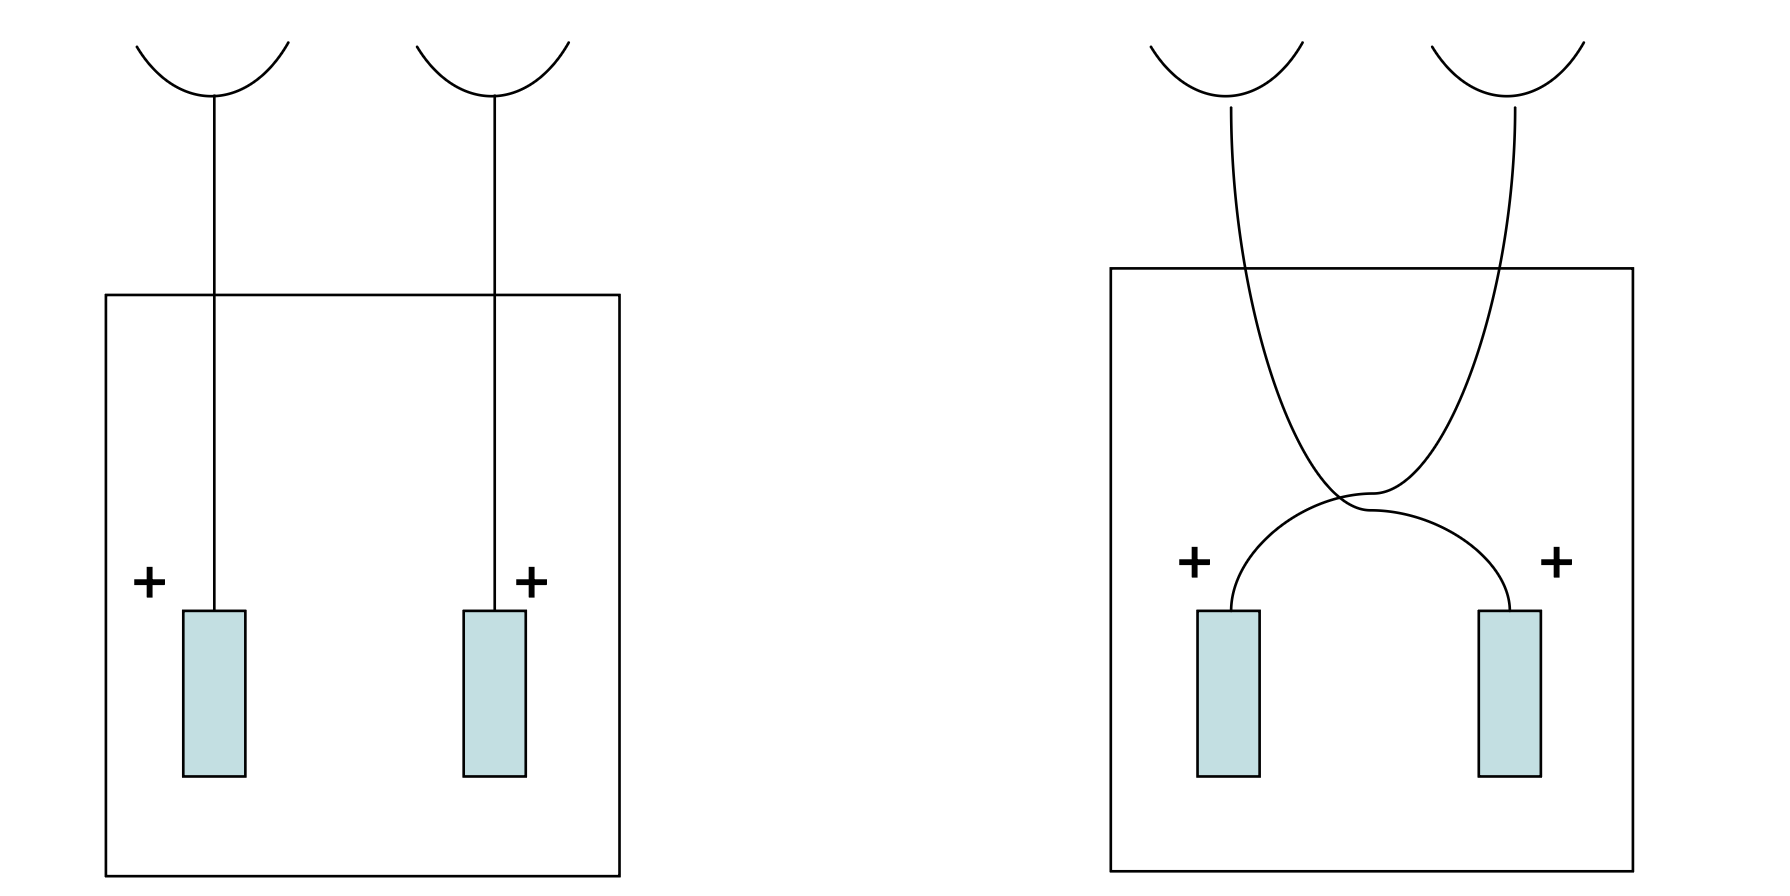
\includegraphics[width = 0.75 \textwidth]{FF/Robotik/Skript/Abbildungen/furchtAgression.png}
\end{center}

Im Bild links ist das Vehikel \enquote{Furcht} abgebildet. Wenn dieses Vehikel eine Lichtquelle entdeckt, zeigt sich das folgende Verhalten:
\begin{itemize}
    \item Befindet sich die Lichtquelle genau in gerader Linie vor dem Vehikel, wird es auf die Lichtquelle zusteuern und immer schneller werden.
    \item Befindet sich die Lichtquelle auf der linken oder rechten Seite des Vehikels, wird dieses sich wegdrehen.
\end{itemize}

\begin{center}
    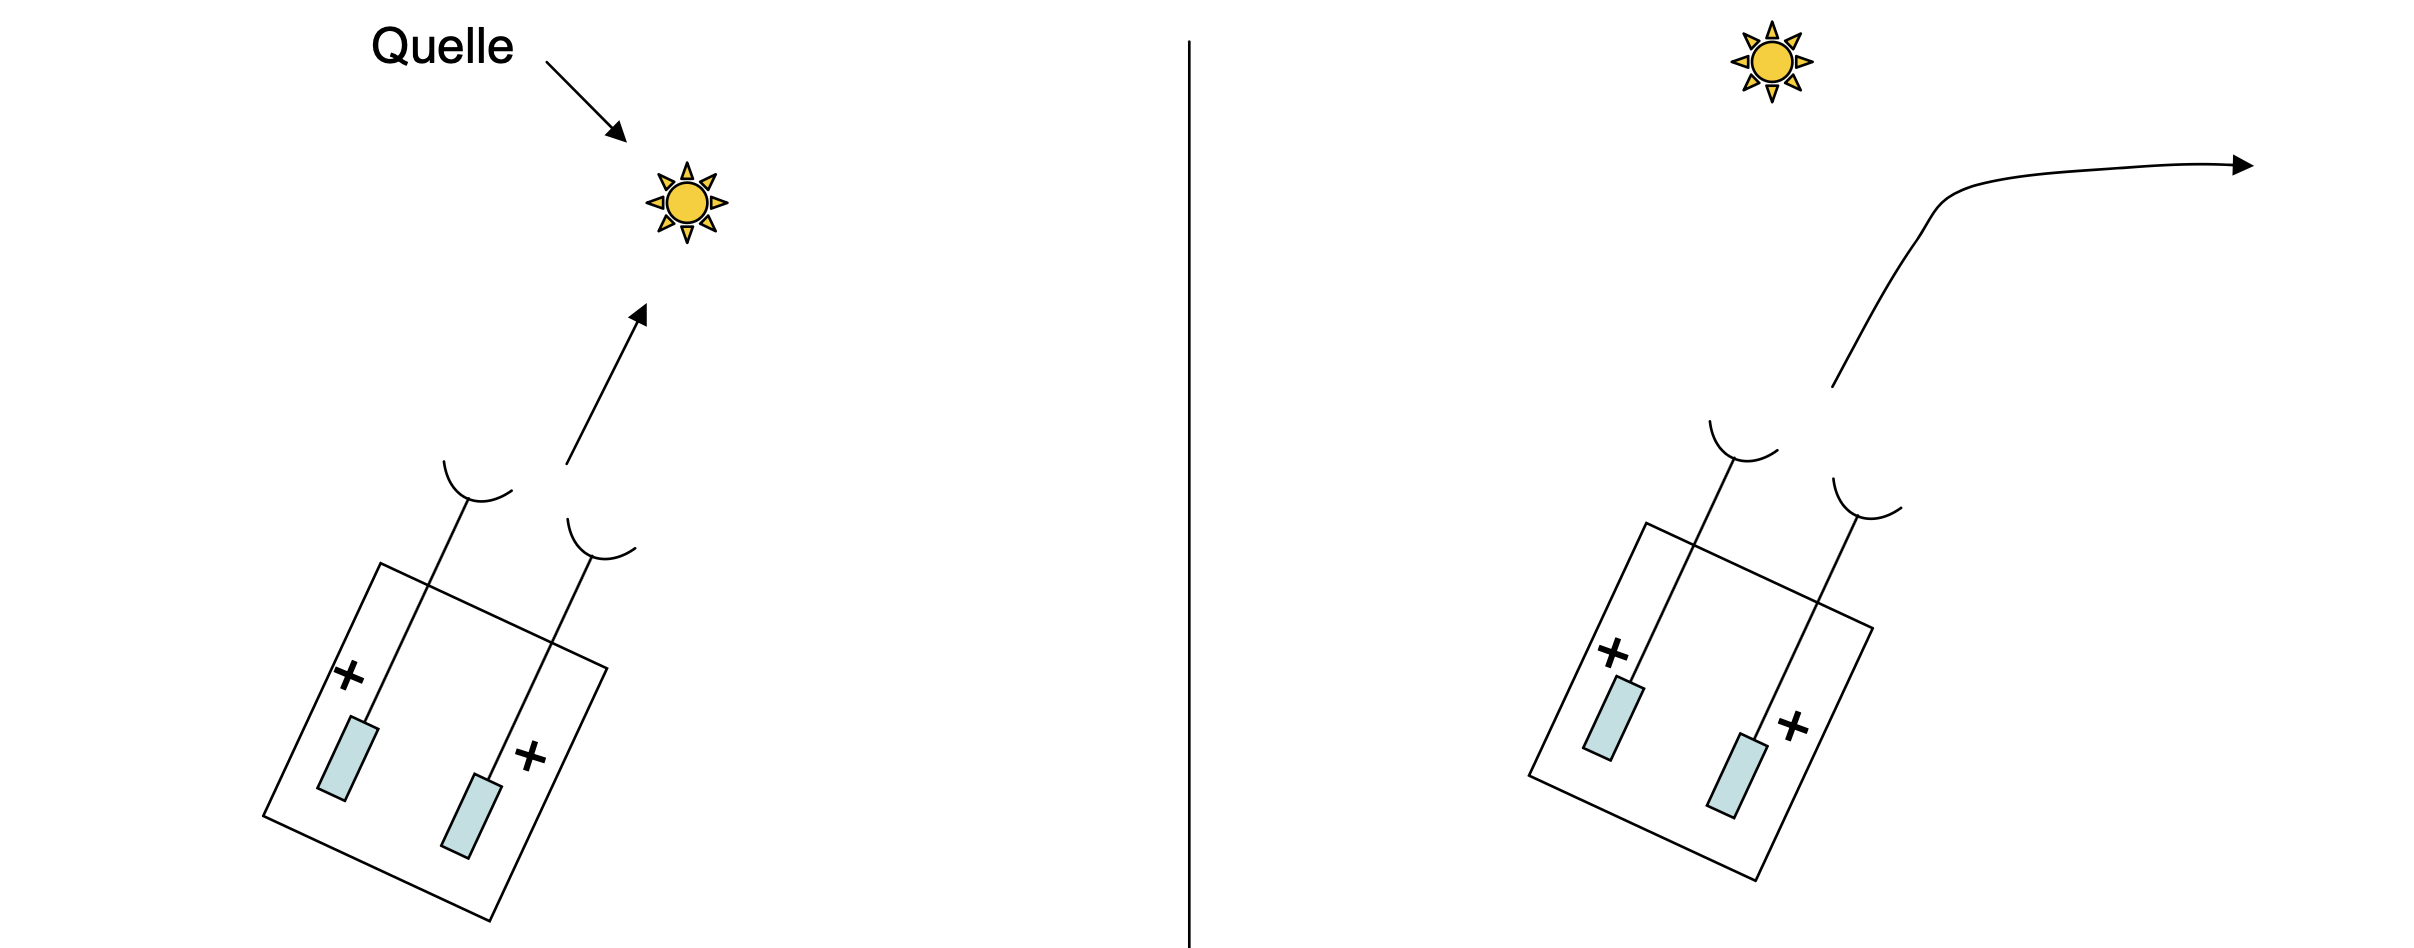
\includegraphics[width = 0.75 \textwidth]{FF/Robotik/Skript/Abbildungen/verhaltenFurcht.png}
\end{center}

Werden Sensoren und Motoren übers Kreuz verbunden, wird das Vehikel \enquote{Aggression} genannt. Das Verhalten ist hier ein anderes:
\begin{itemize}
    \item Befindet sich die Lichtquelle genau in gerader Linie vor dem Vehikel, wird es auf die Lichtquelle zusteuern und immer schneller werden.
    \item Befindet sich die Lichtquelle auf der linken oder rechten Seite des Vehikels, wird dieses zu ihr drehen (und \enquote{angreifen}).
\end{itemize}

\begin{center}
    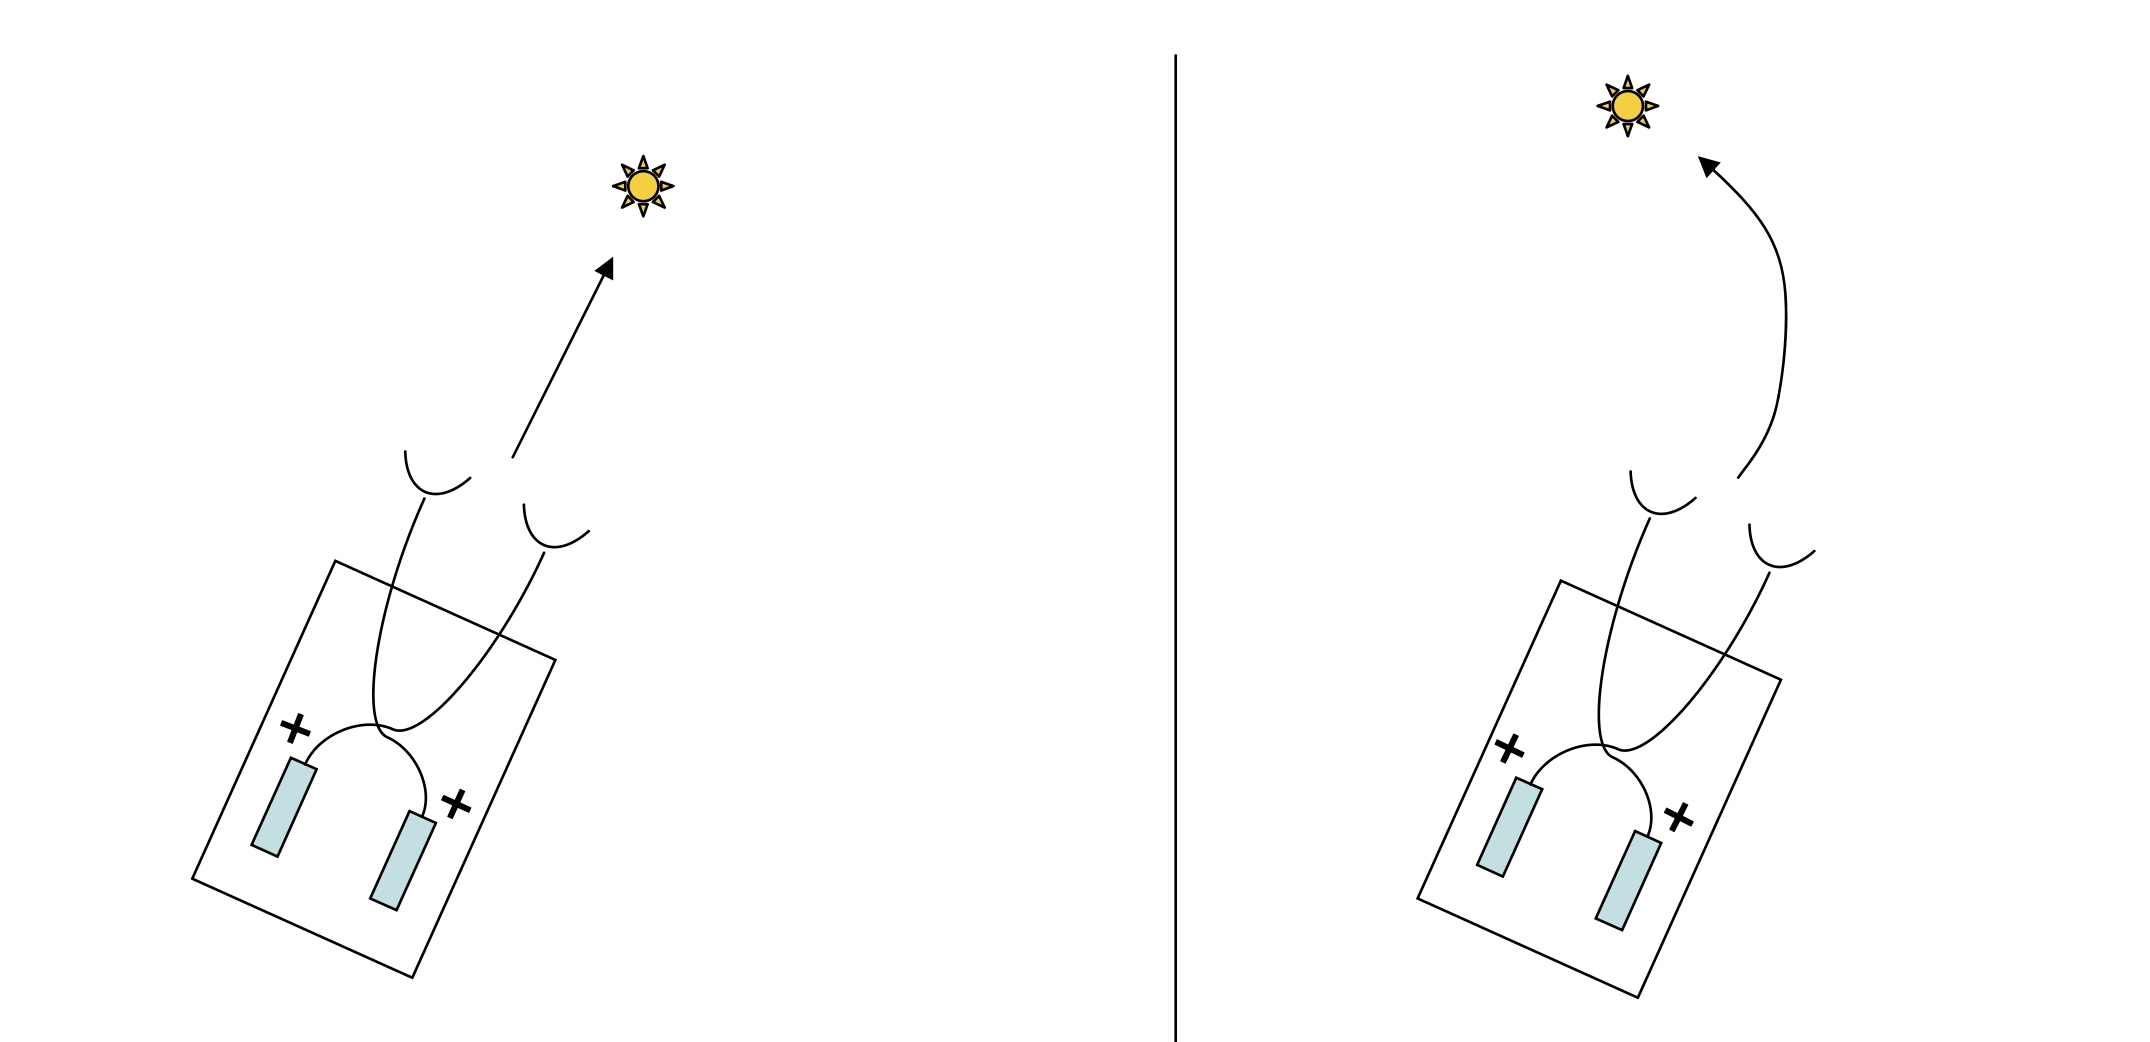
\includegraphics[width = 0.75 \textwidth]{FF/Robotik/Skript/Abbildungen/verhaltenAgro.png}
\end{center}

\begin{myexercise}
    Für diese Aufgabe benötigen Sie ein Braitenberg-Vehikel (anderer Roboter) und eine Lichtquelle.
    \begin{aenum}
        \item Laden Sie den Ordner \texttt{Braitenberg Furcht} von Moodle und testen Sie das Braitenberg-Vehikel.
        \item Schreiben Sie ein Programm für das Braitenberg-Aggression-Vehikel.
    \end{aenum}
\end{myexercise}

\subsection{Ewige und explorative Liebe}

Die Vehikel \enquote{ewige Liebe} und \enquote{explorative Liebe} sind gleich aufgebaut wie \enquote{Furcht} und \enquote{Aggression}. Der einzige Unterschied besteht darin, dass bei den Liebes-Vehikeln die Geschwindigkeit der Motoren \textbf{abnimmt}, je höher der Sensorwert ist.

\enquote{Ewige Liebe} zeigt das folgende Verhalten:
\begin{itemize}
    \item Befindet sich die Lichtquelle genau in gerader Linie vor dem Vehikel, wird es auf die Lichtquelle zusteuern und davor stoppen.
    \item Befindet sich die Lichtquelle auf der linken oder rechten Seite des Vehikels, nähert sich dieses der Quelle und blickt sie (verliebt) an.
\end{itemize}

\begin{center}
    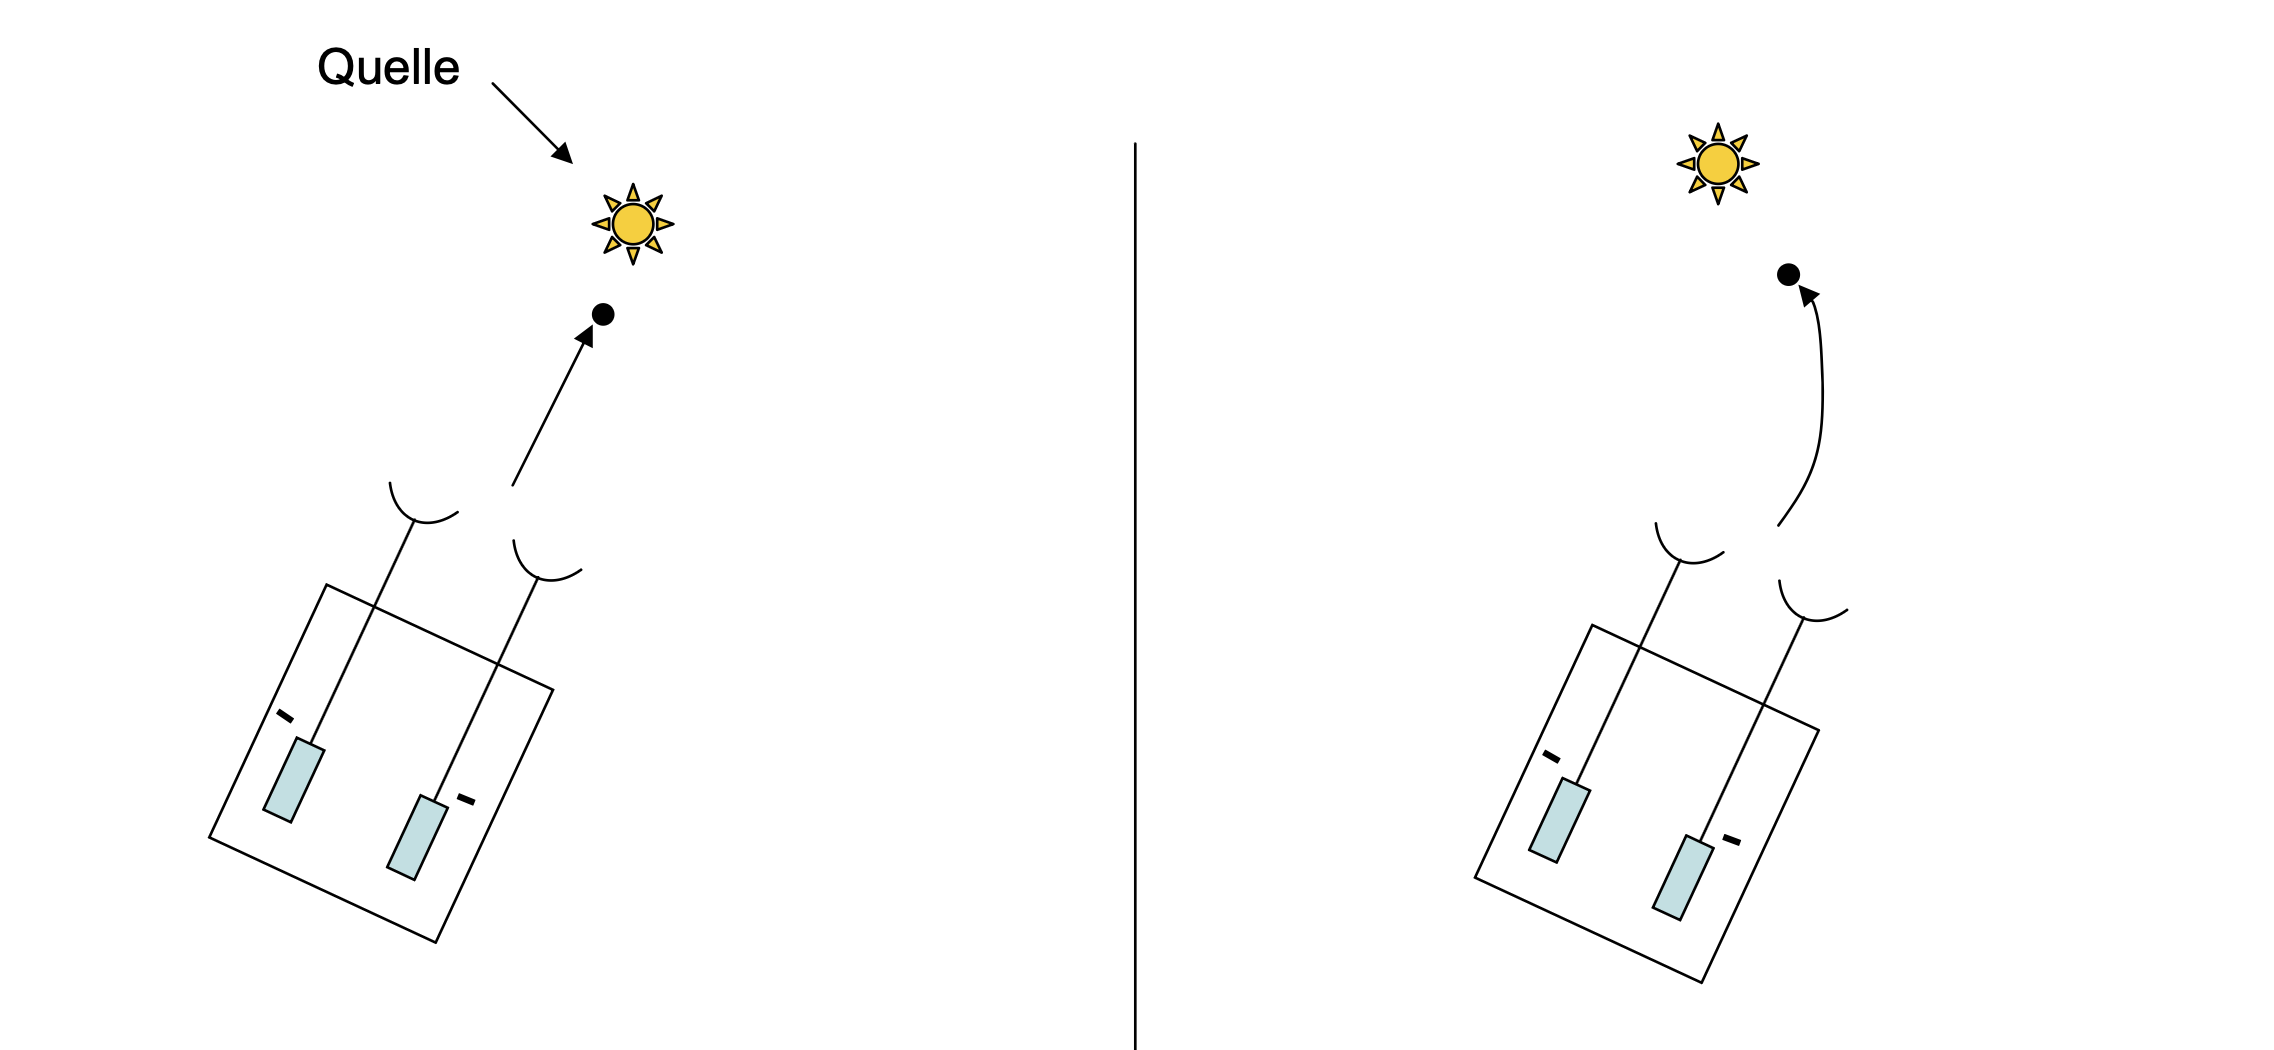
\includegraphics[width = 0.75 \textwidth]{FF/Robotik/Skript/Abbildungen/verhaltenEwigeLiebe.png}
\end{center}

Das Vehikel \enquote{explorative Liebe} verhält sich hingegen so:

\begin{itemize}
    \item Befindet sich die Lichtquelle genau in gerader Linie vor dem Vehikel, wird es auf die Lichtquelle zusteuern und davor stoppen.
    \item Befindet sich die Lichtquelle auf der linken oder rechten Seite des Vehikels, dreht es ab (und sucht eine andere (bessere?) Quelle in der Umgebung).
\end{itemize}

\begin{center}
    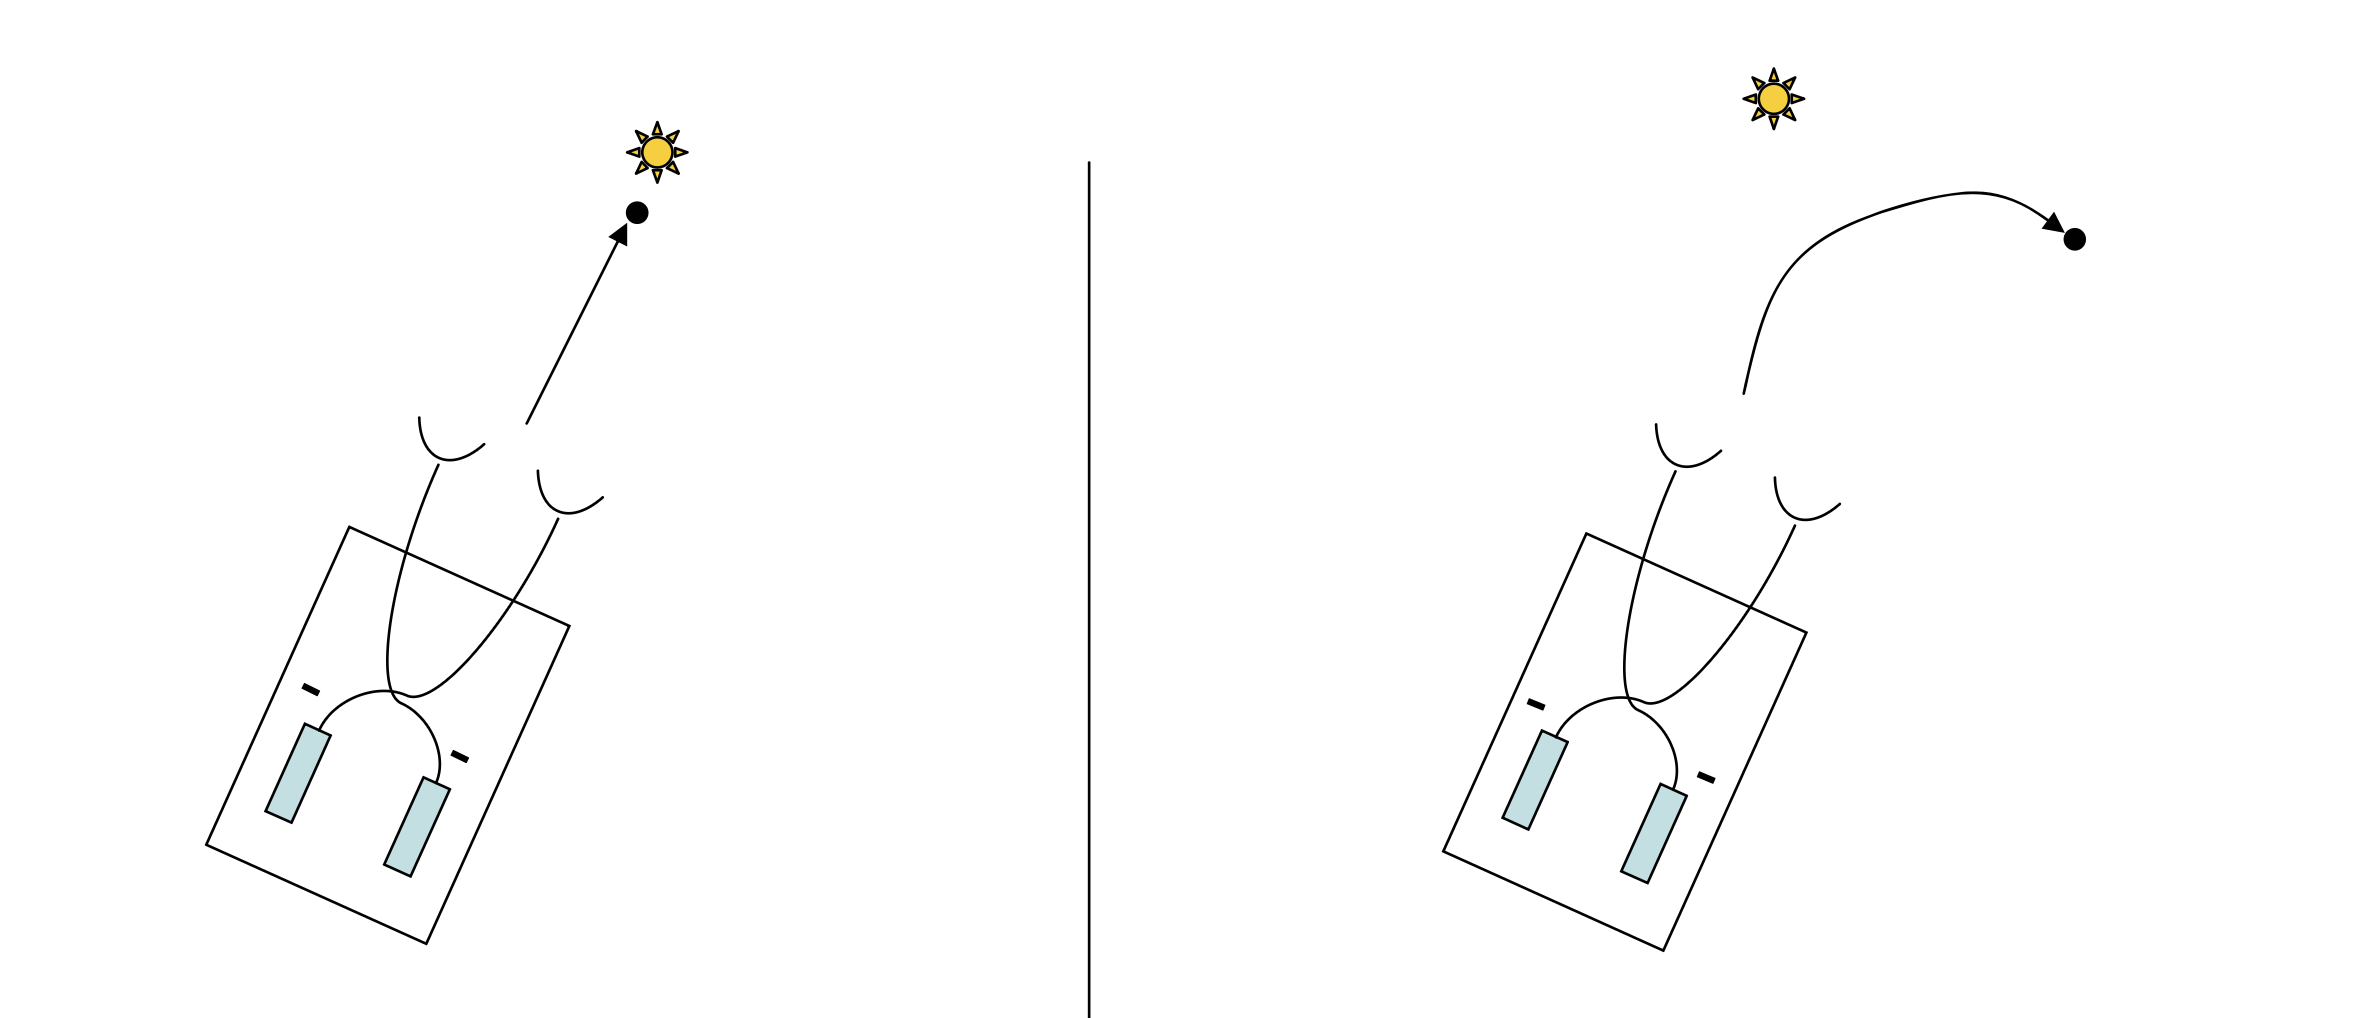
\includegraphics[width = 0.75 \textwidth]{FF/Robotik/Skript/Abbildungen/verhaltenExplorativeLiebe.png}
\end{center}

\begin{myexercise}
    Schreiben Sie für die beiden Vehikel je ein Programm, ausgehend vom Code im Ordner \texttt{Braitenberg Furcht} und beobachten Sie das Verhalten.
\end{myexercise}

\begin{center}
    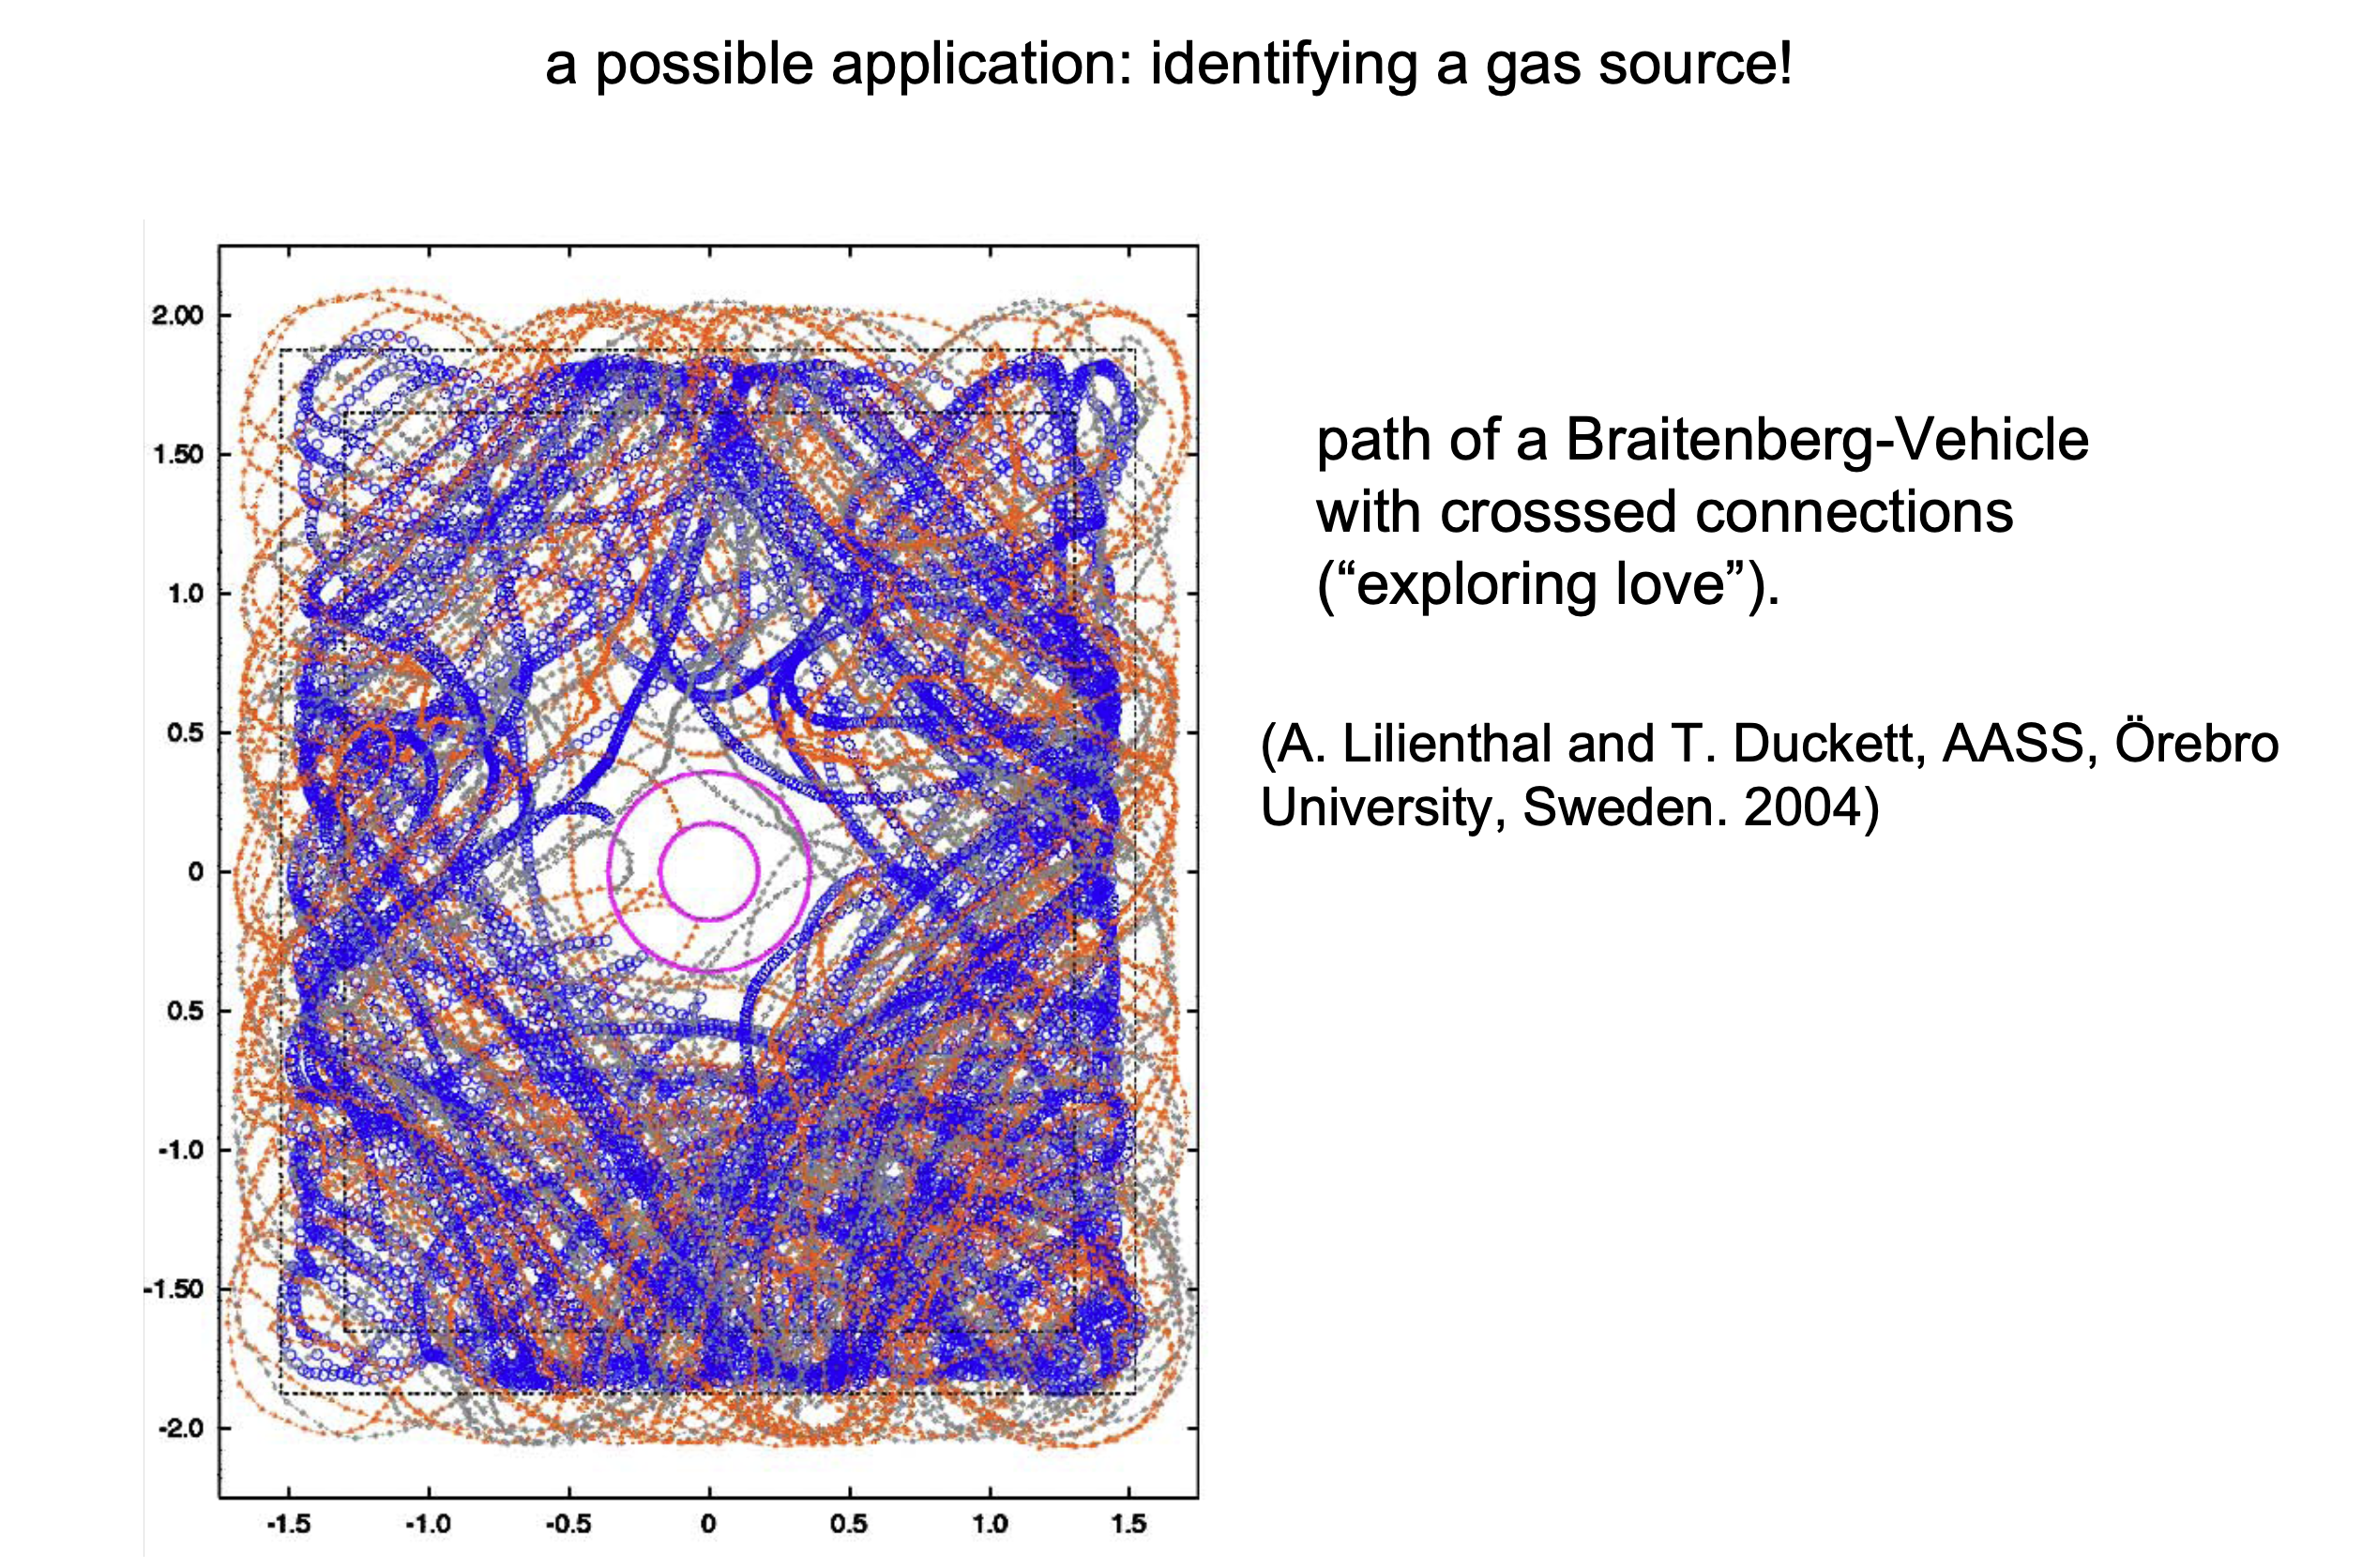
\includegraphics[width = \textwidth]{FF/Robotik/Skript/Abbildungen/identifyingGasSource.png}
\end{center}
